\section{Introduction}
\setcounter{page}{1}
\pagenumbering{arabic}


In this project we are going to find the optimal path for a solar powered airplane \footnote{Like the one from \url{http://www.solarimpulse.com/}}. During flight the plane's electrical engines drain power from it's battery, while at the same time solar panels on the plane's wings convert energy from the sun's rays into electric energy. However clouds may block the sun's rays from reaching the panels. In addition the sun's intensity increases when flying closer to the equator. In order to keep as much energy in the batteries as possible the flight path has to be optimized.

In this paper we will start by explaining the mathematical parameters we have taken into count to calculate the optimal path.
Afterwards we will formulate the problem in it's standard form.
We will finish by presenting some of the results obtained by the optimisation.


\subsection{Formulation of the problem.}

The main goal of this project is to find the best path connecting the starting point of the plane to the destination.
Before this question can be answered we first have to define what we mean by the best path.
We could for instance look at the shortest path, the most sunny path, the fastest path, \dots 
A logical choice to make is to define the best path as the path that yields the most energy, at the end of the flight.

To calculate this energy we  take several parameters in to account like the solar energy, the drag force on the plane and the cost for accelerating the plane.
The combinations of the energy losses and gains will be combined to calculate the best path.
Next we will give a brief explanation about all of these parameters and their mathematical formulation.

\subsubsection{Solar energy}

The solar gain is roughly defined as the amount fo sun than can  be picked up trough the flight.
The local amount of sun is determined by two factors, the angle of the sun at that time and that place and the local cloud density.

For the inclination angle of the sun we used \textbf{\dots STIL TO DO}

To simulate clouds we where looking for highly autocorrelated random data so that the clouds would be located in islands rather than being scattered without any pattern in the sky.
The technique we applied was to generate a low dimensional random matrix and extrapolate the data points to get a continuous grid.
An example of the simulated weather is shown in Figure \ref{fig:RandomWeather}.
The contour lines on this plot represent the cloud densities and the arrows represent the local wind which is generated using the same technique.

At the end the local solar gain is eventually calculated by the product of the suns intensity related to the angle and the amount of clouds.
\begin{equation}
E_{sun}(x,y)  =  V_{sun}(x,y) V_{Cloud}(x,y)
\end{equation}
The total amount of energy collected by the airplane is now given by 
\begin{equation}
E_{sun}(t)  =  -\alpha_{sun}\oint_{path} E_{sun}(x,y)  d\tau,
\end{equation}
this path integral is evaluated over the path from time $ \tau=0 $ until time $ \tau=t $.
The constant term in front of the integral is a scaling term that can be adjusted to tune the weight of the individual energies.
Remark the minus sing in front of the integral, this implies that we want to maximise the solar gain.

\begin{figure}
\centering
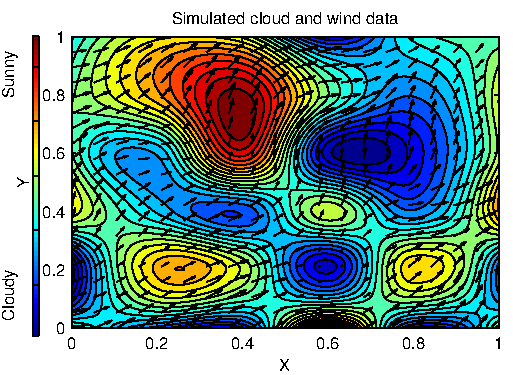
\includegraphics[width=0.5\linewidth]{../src/plot/RandomWeather}
\caption{An example of  simulated weather data. The colour map represents the intensity of the sun, the arrows point in the direction of the wind. This data is created by the  interpolation on a 5 by 5 random generated matrix. }
\label{fig:RandomWeather}
\end{figure}


\subsubsection{Drag resistance}

A second import aspect that influences the energy balance of the airplane is the drag force.
Introducing a drag force will keep the velocity of the plane bounded.
We chose to use a simple quadratic dependency of the drag force and the speed.
This drag force is then defined as,
\begin{equation}
E_{drag}(t)  =  \alpha_{drag} \oint_{path} v(x,y)^2  d \tau.
\end{equation}
In this integral the function $ v(x,y) $ represents the speed of the airplane, all the same conventions for the integral apply as noted above.


\subsubsection{Acceleration force}

The energy needed to accelerate the airplane is the last parameter we looked at.
We did assume there was now energy needed to decelerate the plane which is a realistic approximation for small airplanes.
Ta calculated the acceleration energy we used
\begin{equation}
E_{accel}(t)  =  \alpha_{accel} \oint_{path} s(x,y)^2  d \tau
\end{equation}
In this integral the function $ s(x,y) $ is defined as
\begin{equation}
s(x,y) = 
\begin{cases}
   a(x,y) & \text{if } a(x,y) \geq 0 \\
   0       & \text{if } a(x,y) < 0
  \end{cases}
\end{equation}
Where the function $ a(x,y) $ is the acceleration of the airplane at each point on the path.
The point of integrating the function $ s(x,y) $ is just to get rid of the contribution of the negative acceleration.





